\documentclass{article}
\usepackage{graphicx}

\begin{document}

\title{\LaTeX\ is great}
\author{Bullwinkle}
\date{\today}
\maketitle

\tableofcontents 
\listoffigures

\section{My First Section}

My first document, produced using emacs.  Emacs is nice!
Emacs is also nice for editing \LaTeX.  \LaTeX\ also handles figures
in a very straightforward manner, such as in Figure~\ref{fig:fig01}. %
Figure~\ref{fig:fig01} %
\begin{figure}[t]
  \begin{center}
  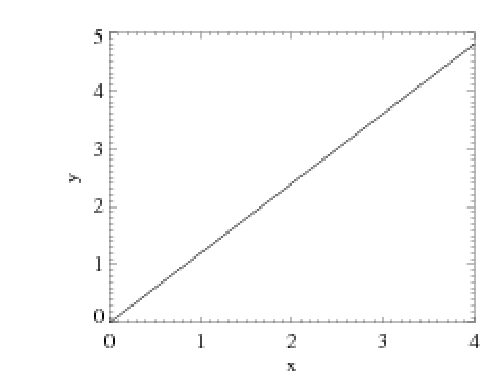
\includegraphics[width=3.75in]{simplefig.pdf}
  \end{center}
  \caption{The caption of the figure.}
\label{fig:fig01}
\end{figure}



\section{On Second Thought}

\LaTeX\ also  produces beautiful mathematics.
\begin{equation}
\psi^\ast = \frac{B(x^\ast)}{\mathrm{Re}_L}\zeta
\end{equation}

\end{document}
